%\usepackage[T1]{fontenc}
%\usepackage[utf8]{inputenc}

%!TEX ROOT=../diploma-thesis.tex

\chapter{Návrh}\label{ch:navrh}

V této kapitole budeme diskutovat návrh frameworku pro centrální správu
a automatickou distribuci business pravidel vyhovující požadavkům identifikovaným
v sekci~\ref{sec:implementation-requirements}. V předchozí kapitole~\ref{ch:reserse}
jsme prozkoumali architektury, které bychom mohli při návrhu využít, a shrnuli
jsme jejich výhody a nevýhody. Došli jsme k závěru, že alternativní přístup \gls{ADDA}
nám poskytne nejlepší aparát pro dosažení vytyčených cílů. Abychom ho mohli plně využít,
je nejprve potřeba formalizovat prostředí \gls{SOA} v rámci \gls{AOP}.

V rámci této kapitoly musíme dále navrhnout vhodný způsob zachycení byznysových pravidel,
jejich uložení a organizaci v rámci systému. Bude potřeba vymyslet proces, jakým budou pravidla
automaticky distribuována.
To bude vyžadovat vytvoření metamodelu, tedy struktury, která bude odpovídat reprezentaci pravidel
v paměti počítače.
Zároveň musíme navrhnout, jakým způsobem budou pravidla vyhodnocována při vykonávání byznysových operací.
Centrální správa pravidel vyžaduje vytyčení procesu, kterým bude možné administrovat
veškerá pravidla v systému tak, aby byla zachována jejich konzistence.

\section{Zachycení byznysových pravidel}

Předpokládáme, že každá služba má lokálně uložen popis byznysových kontextů, které se sémanticky vztahují
k doméně dané služby. Jak jsme již nastínili v sekci~\ref{sec:shortcomings}, služba při výkonu jedné byznysové
operace může potřebovat aplikovat byznysová pravidla, která jsou aplikována také při výkonu jiné byznysové operace
v jiné službě \textendash\xspace tedy patří do byznysového kontextu této další služby. Při použití konvenčního
přístupu bychom tak znovupoužité pravidlo museli zařadit a

% TODO: popsat jak a kde budou pravidla uložena

\section{Formalizace architektury orientované na služby}

V kapitole~\ref{ch:analyza} jsme již identifikovali, jaké průřezové problémy, resp. aspekty,
jsou řešeny v informačních systémech a dospěli jsme k závěru, že byznysová pravidla jsou
jejich významným zástupcem. V sekci ~\ref{sec:shortcomings} jsme shrnuli konkrétní
problémy byznysových pravidel, které konvenční přístup neumí v rámci \gls{SOA} efektivně řešit.
Pro formalizaci \gls{SOA} do termínů \gls{AOP} musíme ještě identifikovat \textit{join-points},
ve kterých je možné aspekty v podobě byznysových pravidel aplikovat. Dále je potřeba určit podobu
\textit{advices}, popsat způsob jakým budou zachyceny \textit{pointcuts} a také navrhnout proces
\textit{weavingu} pravidel.

\subsection{Join-points}

Při identifikování join-points budeme vycházet ze životního cyklu služby, který je znázorněn
na obrázku~\ref{fig:join-points}. První fází v životě instance služby je její inicializace,
konkrétně načtení aplikačního kontextu. V tomto bodě je potřeba získat veškerá pravidla, která ... % TODO: fixme

Ve chvíli, kdy je inicializace služby hotova, vstupuje do fáze, ve které může přijímat požadavky
na vykonání byznysových operací. Pokud služba přijme takový požadavek, je nejprve nutno určit
byznysový kontext a vyhodnotit veškeré \textit{preconditions}. Pokud jsou všechny předpoklady
pro spuštění operace splněny, může být vykonána. Po dokončení operace je nutno aplikovat relevantní
post-conditions.

\begin{figure}
    \centering
    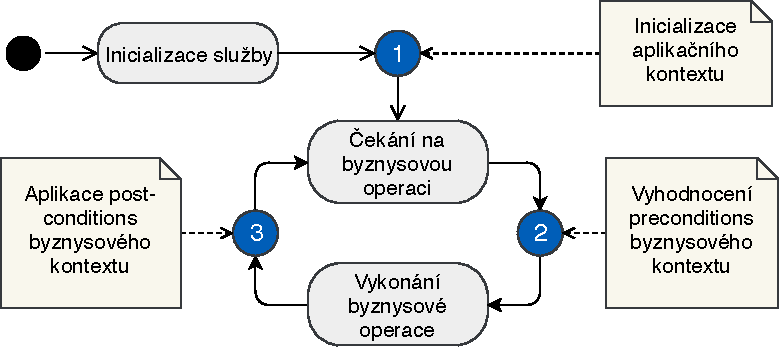
\includegraphics[keepaspectratio=true, width=0.8\linewidth]{figures/join-points.pdf}
    \caption{Diagram životn\'{\i}ho cyklu služby a identifikovan\'ych join-pointů}
    \label{fig:join-points}
\end{figure}

Identifikované join-points tedy jsou:

\benum[label=\circledarabic]
\item\label{itm:initialization} Inicializace instance služby
\item\label{itm:before} Start byznysové operace
\item\label{itm:after} Dokončení byznysové operace
\eenum

\subsection{Pointcuts}

V join-pointu~\ref{itm:initialization} by služba měla načíst všechny byznysové kontexty, které
bude potřebovat ke své činnosti, a nejsou pro ni lokálně dostupné. Služba tedy musí zjistit,
která pravidla je potřeba získat, a následně si je vyžádat od ostatních služeb.
V join-pointech~\ref{itm:before}~a~\ref{itm:after} musejí být aplikována byznysová pravidla každého
kontextu vztahujícího se k dané operaci.

Nyní je potřeba se zamyslet, jakým způsobem budou selektory join-pointů pro jednotlivé kontexty zapsány.
Pokud bychom chtěli u každého byznysového kontextu zapsat, ke kterým byznysovým operacím se vztahuje,
museli bychom předem znát seznam veškerých byznysových operací implementovaných v celém systému. Pokud si
představíme příklad ze sekce~\ref{sec:shortcomings}, musela by služba implementující vystavování
faktur předem vědět o všech případech, kde bude potřeba validovat validační adresu, aby tato místa mohla
adresovat. To ovšem není příliš vhodné řešení.

\begin{figure}
    \centering
    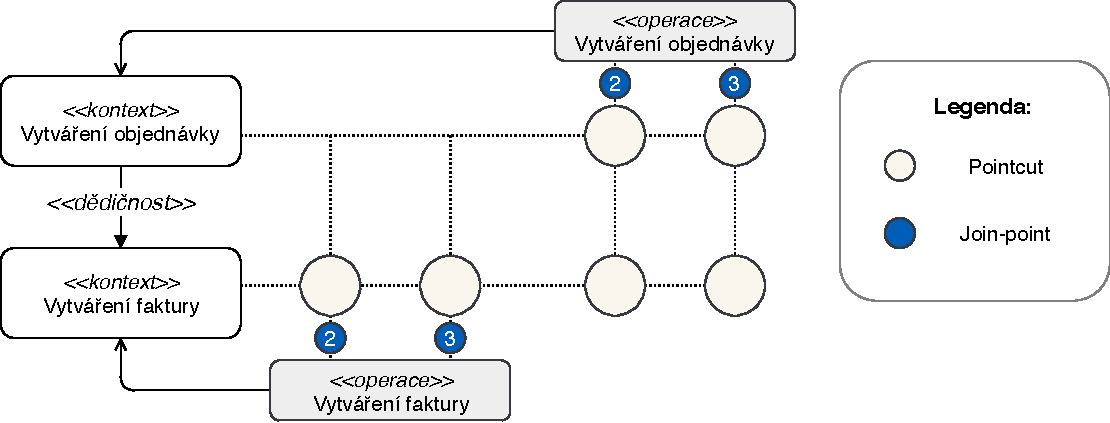
\includegraphics[keepaspectratio=true, width=1\linewidth]{figures/context-extension.pdf}
    \caption{Diagram znázorňující dědičnost kontextů ve vztahu k join-pointům a pointcuts}
    \label{fig:context-extension}
\end{figure}

Lepším způsobem zápisu, který přirozeně odpovídá směru mezi byznysovými kontexty služeb,
je přidání konceptu dědičnosti kontextů. Každý kontext, který by potřeboval validovat fakturační
adresu, by tak mohl pouze dědit od kontextu vytváření faktury. Byznysové operaci by pak stačilo
odkázat se na byznysový kontext, který využívá. Na obrázku~\ref{fig:context-extension} můžeme vidět,
jak by takový případ mohl vypadat. Kontext vytváření objednávky dědí od kontextu vytváření faktury
a sdílí tak jeho byznysová pravidla. Byznysové operace se odkazují, které byznysové kontexty mají
být při jejich vykonávání použity. Jak můžeme vidět, před spuštěním a po dokončení operace vytváření
objednávky jsou aplikována pravidla obou kontextů, zatímco při vytváření faktury jsou zohledněna
pouze pravidla jednoho kontextu.

\subsection{Advices}

V případě join-pointu~\ref{itm:initialization} se za advice dá považovat repretenzace byznysového
kontextu přenášeného mezi službami. Naopak v join-pointech~\ref{itm:before}~a~\ref{itm:after}
je přidanou funkcionalitou vyhodnocování preconditions nad aplikačním kontextem, resp. aplikování
post-conditions na návratovou hodnotu operace.

\subsection{Weaving}

Weaving v případě join-pointu~\ref{itm:initialization} provádí komponenta frameworku, která
analyzuje lokálně dostupná pravidla služby, vyhodnotí, která pravidla je potřeba stáhnout,
a vyžádá pravidla od příslušných služeb.

V případě join-pointů~\ref{itm:before}~a~\ref{itm:after} se o weaving postará jiná komponenta.
Ta musí zachytit volání byznysové operace a získat informace o aktuálním stavu aplikačního kontextu.
Následně zjistí, který byznysový kontext má být aplikován, shromaždí všechna preconditions
a každou z nich vyhodnotí. Pokud některá precondition není splněna, byznysová operace je zastavena
a je vyhozena výjimka, na kterou musí služba reagovat. V opačném případě je kontrola vrácena zpět
službě, která vykoná byznysovou operaci. Po jejím skončení opět přichází na aspect weaver, který
zachytí výstup byznysové operace a aplikuje post-conditions daného byznysového kontextu.

\section{Dědičnost byznysových kontextů}

\section{Architektura frameworku}

\section{Zachycen\'{\i} byznysového konextu}

Př\'{\i}stup \gls{ADDA} doporučuje popsat byznysová pravidla pomoc\'{\i}
vlastn\'{\i}ho, na m\'{\i}ru šitého, doménově specifického jazyka~\cite{cemus2015automated}.
V našem př\'{\i}padě můžeme jazykem \gls{DSL} popsat kompletně i cel\'y
byznysov\'y kontext.

V sekci~\ref{sec:business-rule-dsl} jsme zjistili, že ačkoliv jsou nástroje Drools a JetBrains
MPS velmi silnými aparáty, jejich vlastnosti nejsou plně vhodné pro řešení problému
centrální administrace a automatické distribuce byznysových pravidel.
Můžeme jít cestou volby co nejvhodnějšího jazyka pro každou platformu, kterou chceme
využívat pro naše účely, a implementace adapterů pro tyto jazyky, které transformují
dané \gls{DSL} do reprezentace vhodné pro využití naším frameworkem. Vzhledem k
různým vlastnostem těchto jazyků by takový přístup byl suboptimální.

\section{Metamodel byznys kontextu}\label{sec:metamodel}

\begin{figure}
    \centering
    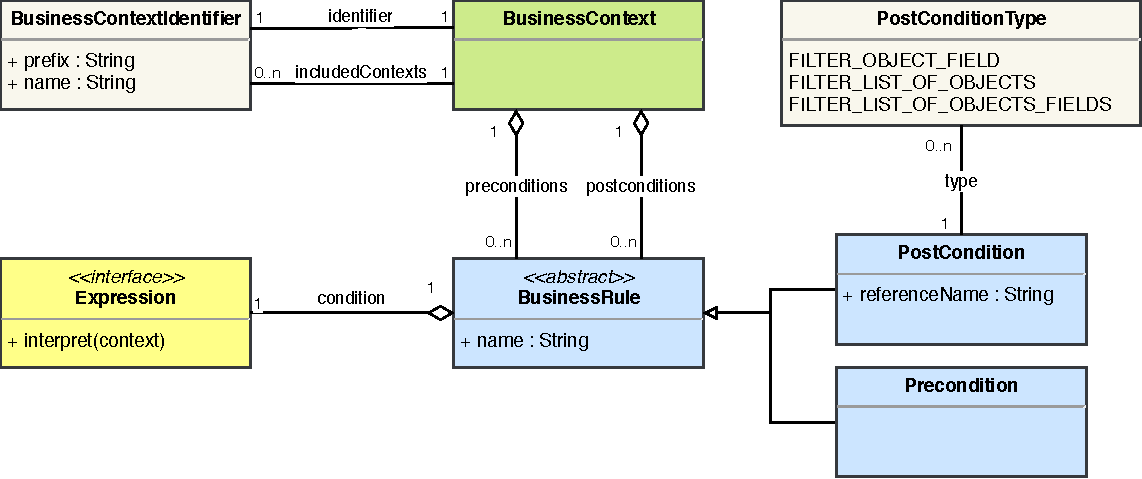
\includegraphics[keepaspectratio=true, width=\linewidth]{figures/business-context-metamodel.pdf}
    \caption{Diagram tř\'{\i}d metamodelu byznysového kontextu}
    \label{fig:business-context-metamodel}
\end{figure} % TODO: popsat

\section{Expression}

\section{Registr byznys kontextů}

\begin{figure}
    \centering
    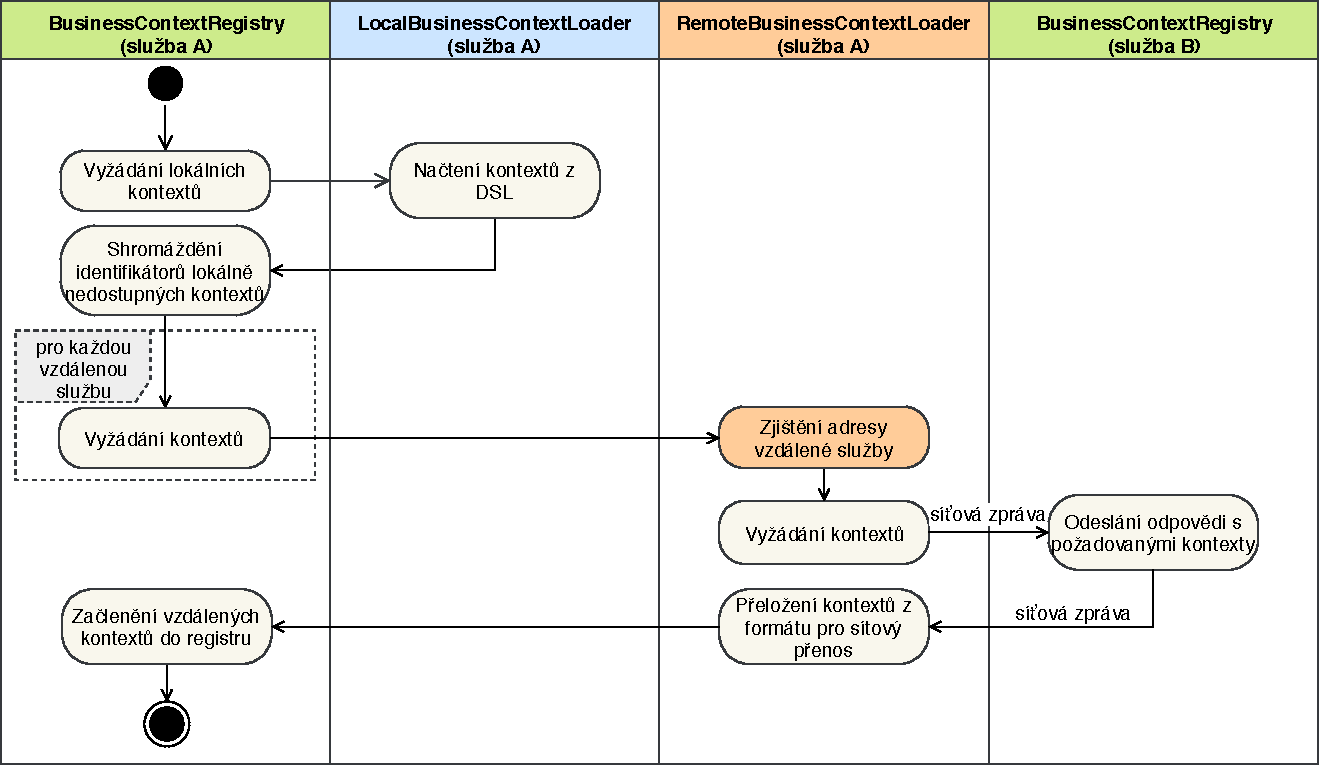
\includegraphics[keepaspectratio=true, width=0.8\linewidth]{figures/business-context-loading.pdf}
    \caption{Diagram procesu inicializace byznysov\'ych kontextů}
    \label{fig:business-context-loading}
\end{figure} % TODO: popsat

\section{Byznys kontext weaver}

\begin{figure}
    \centering
    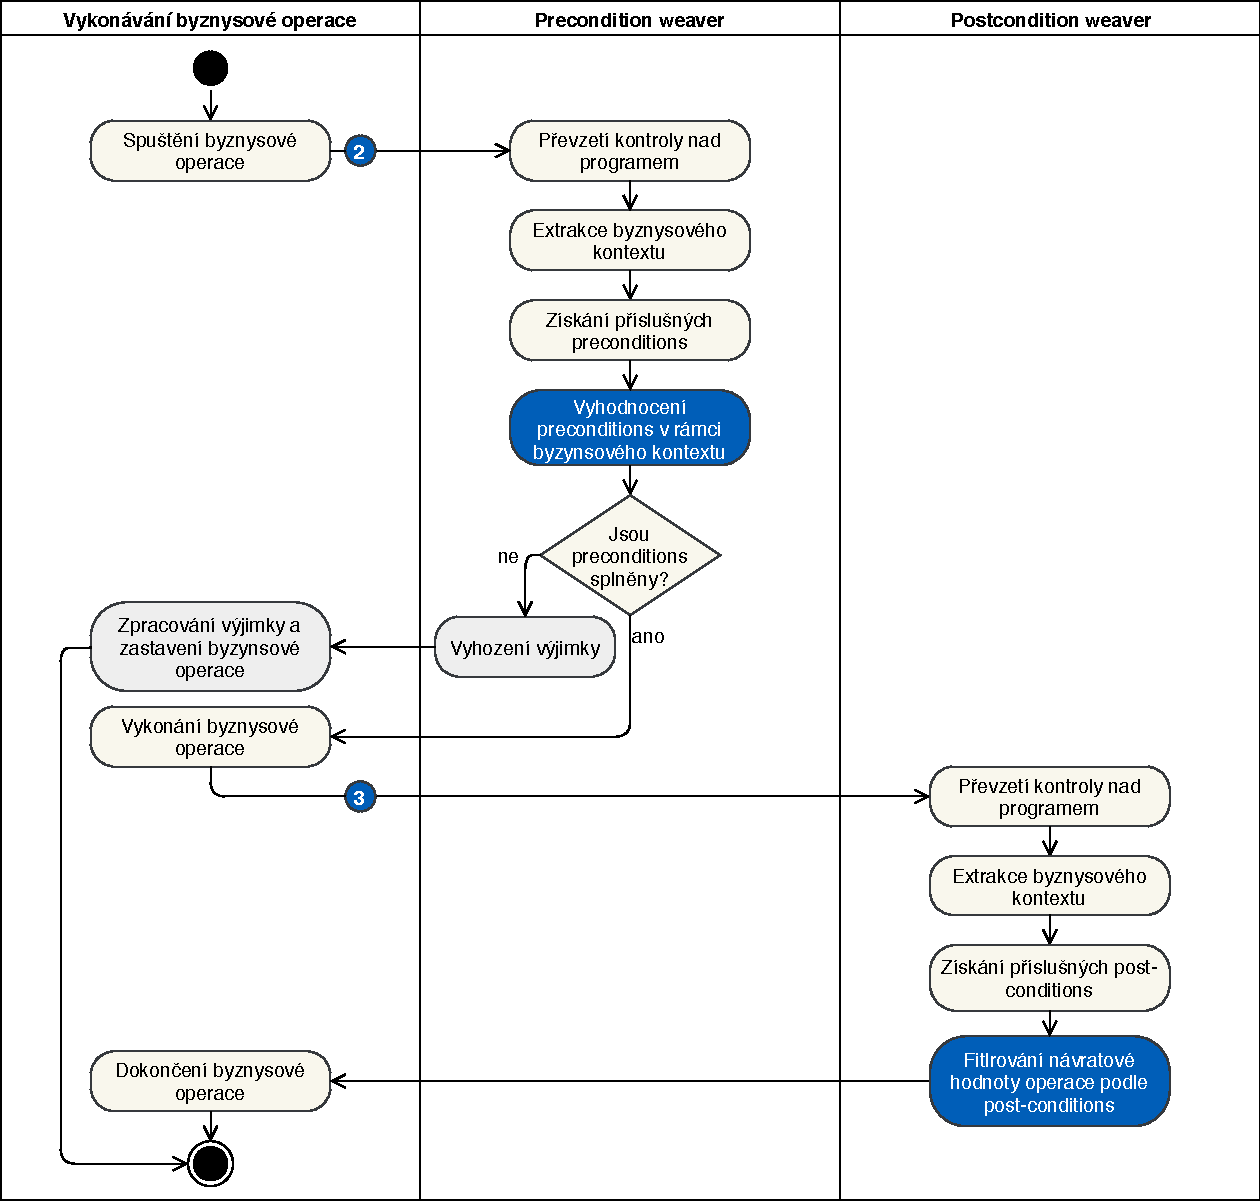
\includegraphics[keepaspectratio=true, width=0.8\linewidth]{figures/business-rules-weaver.pdf}
    \caption{Diagram aktivit weaverů byznysov\'ych pravidel}
    \label{fig:business-rules-weaver}
\end{figure} % TODO: popsat

\section{Centráln\'{\i} správa byznys kontextů}

Vzhledem k nutnosti centralizovat správu byznysových kontextů se nám
architektura \gls{P2P} představená v subsekci~\ref{sec:p2p} nehodí.
Při úpravě kotextů by totiž v systému mohly existovat staré i nové verze
byznysových pravidel, což je pro správnou funkci systém nepřijatelné.
Využijeme tedy architektury klient-server s více servery.
Byznysové kontexty budou podle svého prefixu rozděleny do skupin
a každou ze skupin bude spravovat jedna služba, která bude zároveň
držet jejich aktuální a jediný stav.

\begin{figure}
    \centering
    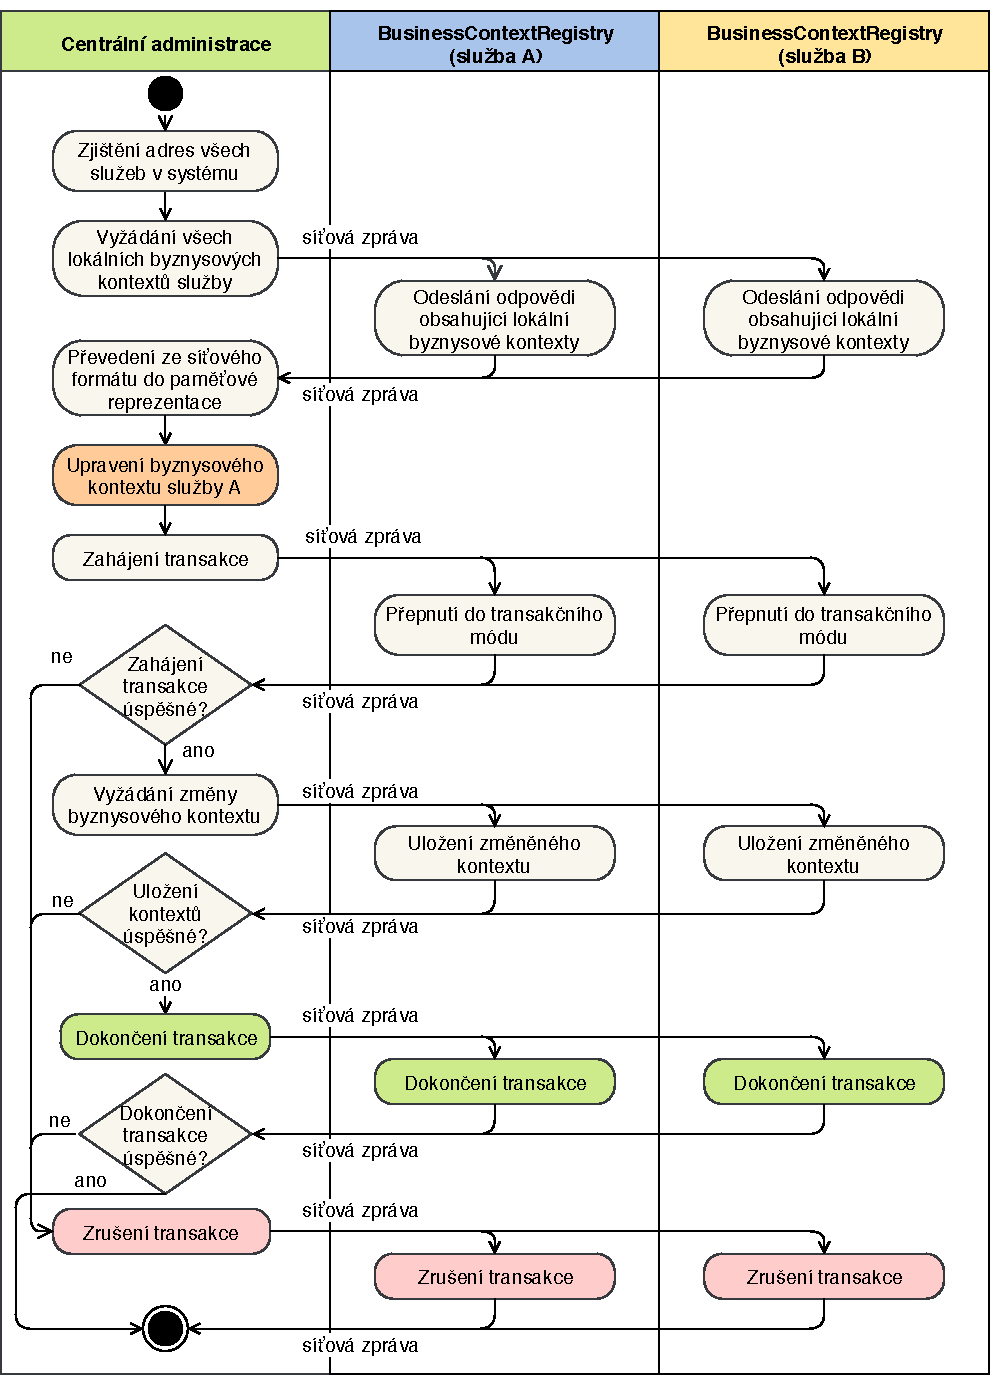
\includegraphics[keepaspectratio=true, width=0.8\linewidth]{figures/business-context-management.pdf}
    \caption{Diagram procesu centráln\'{\i} správy byznysov\'ych kontextů}
    \label{fig:business-context-management}
\end{figure} % TODO: popsat

\subsection{Uložen\'{\i} rozš\'{\i}řeného pravidla}

\goal{Diskutovat chaining vs. direct update}
% TODO: napiš mě

\section{Service discovery}

% TODO: visitor pro uložení pravidla
% TODO: composite strom expressions
% TODO: interpreter pro vyhodnocení expressions

\goal{Popsat nezávislost na service discovery}
